%%%%%%%%%%%%%%%%%%%%%%%%%%%%%%%%%%%%%%%%%%%%%%%%%%%%%%%%
% Este é um documento que servirá de modelo para
% os relatórios feitos na disciplina Laboratório de Circuitos Lógicos
% 2020-2
%%%%%%%%%%%%%%%%%%%%%%%%%%%%%%%%%%%%%%%%%%%%%%%%%%%%%%%%%

%%%%%%%%%%%%%%%%%%%%%%%%%%%%%%%%%%%%%%%%%%%%%%%%%%%%%%%%%
% Use os diferentes diretórios para colocar os relatórios de cada experimento, deste modo vc consegue manter um histórico e todo material organizado em apenas um local.
% Lembre-se de mudar o Main Document no Menu!!!

\documentclass[12pt]{article}

\usepackage{sbc-template}
\usepackage[brazil,american]{babel}
\usepackage[utf8]{inputenc}

\usepackage{graphicx}
\usepackage{url}
\usepackage{float}
\usepackage{listings}
\usepackage{color}
\usepackage{todonotes}
\usepackage{algorithmic}
\usepackage{algorithm}
\usepackage{hyperref}
\usepackage{amsmath}
\usepackage{graphicx}
\usepackage{array}
\usepackage[shortlabels]{enumitem}

\sloppy


\title{Experimento 5\\
Circuitos Combinacionais: Codificador e Decodificador}

\author{Matheus Cardoso de Souza, 202033507\\
        Ualiton Ventura da Silva, 202033580\\
        Grupo G42
}

%%%% LEMBRE-SE DE MUDAR O GRUPO NA LINHA ABAIXO!!!!! %%%%%%
\address{Dep. Ciência da Computação -- Universidade de Brasília (UnB)\\
  CIC0231 - Laboratório de Circuitos Lógicos
  \email{matheus-cardoso.mc@aluno.unb.br, 202033580@aluno.unb.br}
}

\begin{document}
\maketitle

\selectlanguage{american}
 \begin{abstract}
   TODO
 \end{abstract}
\selectlanguage{brazil}

 \begin{resumo}
   TODO
 \end{resumo}


\section{Introdução}
\label{sec:Introducao}

% Escreva com suas palavras o que vai ser trabalhado no experimento. Aqui temos um exemplo de como citar a bibliografia consultada \cite{boulic:91} \cite{smith:99}.

TODO

\subsection{Objetivos}
\label{sec:Objetivos}

TODO

\subsection{Materiais}
\label{sec:Materiais}
Em função da natureza do ensino a distância, os presentes experimentos não foram
realizados usando-se materiais e equipamentos físicos, mas sim emulados por meio
do \href{https://www.digitalelectronicsdeeds.com/deeds.html}{Deeds}.

A seguir estão enumerados os materiais utilizados:
\begin{itemize}
        TODO
\end{itemize}

\section{Procedimentos}
\label{sec:Procedimentos}
% \setcounter{subsection}{-1}

Passaremos a apresentar os experimentos requeridos.

% 2.1
\subsection{Elaboração de Codificador}\label{sec:elaboração_codificador}

Para a elaboração do circuito, deve-se analisar a seguinte tabela:
\begin{table}[H]
    \centering
    \caption{}
    \begin{tabular}{|c|c|c|c|c|}\hline
    \multicolumn{1}{|c|}{Entrada} & \multicolumn{4}{|c|}{Saida} \\\hline
    \textbf{$ $} & \textbf{$A$} & \textbf{$B$} & \textbf{$C$} & \textbf{$D$} \\\hline
    0 & 0 & 0 & 0 & 0 \\\hline
    1 & 0 & 0 & 0 & 1\\\hline
    2 & 0 & 0 & 1 & 1\\\hline
    3 & 0 & 0 & 1 & 0\\\hline
    4 & 0 & 1 & 1 & 0\\\hline
    5 & 0 & 1 & 1 & 1\\\hline
    6 & 0 & 1 & 0 & 1\\\hline
    7 & 0 & 1 & 0 & 0\\\hline
    8 & 1 & 1 & 0 & 0\\\hline
    9 & 1 & 1 & 0 & 1\\\hline
    \end{tabular}\label{tab:comparador_de_palavras_3_bits}
\end{table}

Sendo que '0' é codificado como '0000000001', '1' como '0000000010', ... , '9' como '1000000000'.
Temos que para cada 10 bits de entrada temos que somente 1 será dado como 1, por exemplo, não temos a entrada '0000000011'.

Denotando cada um dos 10 bits como $e_{9},e_{8},e_{7},e_{6},e_{5},e_{4},e_{3},e_{2},e_{1},e_{0}$. Assim, deve-se analisar também que cada bit também descreve seu respectivo valor, exemplo, $e_{8}$ descreve o símbolo '8', pois, quando $e_{8}=1$ temos que todos os outros serão iguais a 0, portanto, estaremos descrevendo o valor '8'.

Para maior simplicidade podemos analisar o fato de que para a saída \textbf{$A$}, depende de somente as entradas $e_{8}$ e $e_{9}$, como cada caso irá ocorrer de maneira individual, \textbf{$A$} poderá ser descrito como:
\begin{equation}
F_{A}(e_{8}, e_{9}) = e_{8} + e_{9}
\end{equation}

Utilizando raciocínio semelhante para outros, temos então que:

\begin{equation}
F_{B}(e_{4},e_{5},e_{6},e_{7},e_{8}) = e_{4}+e_{5}+e_{6}+e_{7}+e_{8}
\end{equation}

\begin{equation}
F_{C}(e_{2},e_{3},e_{4},e_{5}) = e_{2}+e_{3}+e_{4}+e_{5}
\end{equation}

\begin{equation}
F_{D}(e_{1},e_{2},e_{5},e_{6},e_{9}) = e_{1}+e_{2}+e_{5}+e_{6}+e_{9}
\end{equation}

\begin{figure}[htp]
    \centering
    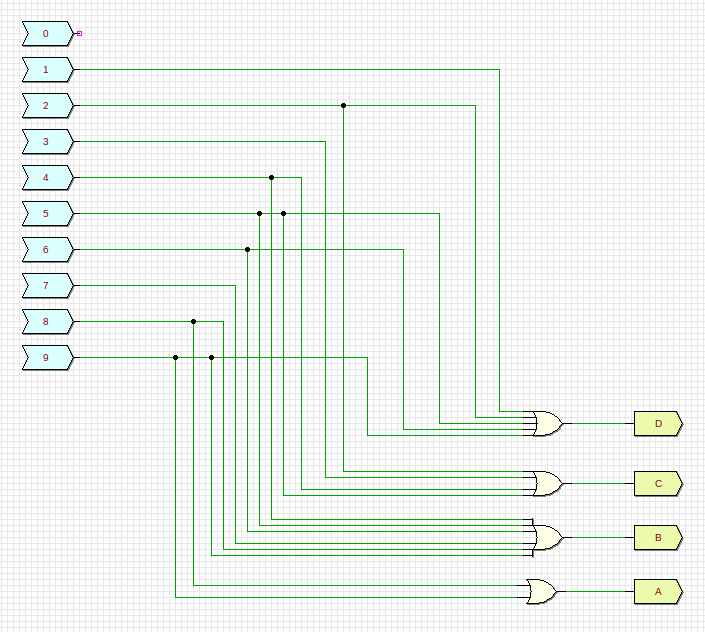
\includegraphics[width=12cm]{Exp05/2.1.png}
    \caption{Subcircuito Comparador}
    \label{fig:galaxy}
\end{figure}


% 2.3
\subsection{Obtendo as funções booleandas para o decodificador}\label{sec:boolean_functions_decoder}

Nesta seção temos por objetivo obter as funções booleanas para o decodificador
de números em código decimal para números em código de Gray.

\begin{table}[H]
    \centering
    \caption{Tabela Verdade para o Decodificador}
    \begin{tabular}{|c|c|c|c||c|c|c|c|c|c|c|c|c|c|}\hline
    \multicolumn{4}{|c||}{Entradas} & \multicolumn{10}{|c|}{Saídas} \\\hline
    \textbf{A} & \textbf{B} & \textbf{C} & \textbf{D} & \textbf{0} & \textbf{1} & \textbf{2} & \textbf{3} & \textbf{4} & \textbf{5} & \textbf{6} & \textbf{7} & \textbf{8} & \textbf{9} \\\hline
    0 & 0 & 0 & 0 & 1 & 0 & 0 & 0 & 0 & 0 & 0 & 0 & 0 & 0 \\\hline
    0 & 0 & 0 & 1 & 0 & 1 & 0 & 0 & 0 & 0 & 0 & 0 & 0 & 0 \\\hline
    0 & 0 & 1 & 1 & 0 & 0 & 1 & 0 & 0 & 0 & 0 & 0 & 0 & 0 \\\hline
    0 & 0 & 1 & 0 & 0 & 0 & 0 & 1 & 0 & 0 & 0 & 0 & 0 & 0 \\\hline
    0 & 1 & 1 & 0 & 0 & 0 & 0 & 0 & 1 & 0 & 0 & 0 & 0 & 0 \\\hline
    0 & 1 & 1 & 1 & 0 & 0 & 0 & 0 & 0 & 1 & 0 & 0 & 0 & 0 \\\hline
    0 & 1 & 0 & 1 & 0 & 0 & 0 & 0 & 0 & 0 & 1 & 0 & 0 & 0 \\\hline
    0 & 1 & 0 & 0 & 0 & 0 & 0 & 0 & 0 & 0 & 0 & 1 & 0 & 0 \\\hline
    1 & 1 & 0 & 0 & 0 & 0 & 0 & 0 & 0 & 0 & 0 & 0 & 1 & 0 \\\hline
    1 & 1 & 0 & 1 & 0 & 0 & 0 & 0 & 0 & 0 & 0 & 0 & 0 & 1 \\\hline
    \end{tabular}\label{tab:tabela_and}
\end{table}

Analisando a tabela verdade, é fácil verificarmos quais devem ser as funções
booleanas de cada saída. Reproduzimos em seguida cada uma delas:

\begin{align}
0 &= \overline{A} \cdot \overline{B} \cdot \overline{C} \cdot \overline{D} \\
1 &= \overline{A} \cdot \overline{B} \cdot \overline{C} \cdot D \\
2 &= \overline{A} \cdot \overline{B} \cdot C \cdot D \\
3 &= \overline{A} \cdot \overline{B} \cdot C \cdot \overline{D} \\
4 &= \overline{A} \cdot B \cdot C \cdot \overline{D} \\
5 &= \overline{A} \cdot B \cdot C \cdot D \\
6 &= \overline{A} \cdot B \cdot \overline{C} \cdot D \\
7 &= \overline{A} \cdot B \cdot \overline{C} \cdot \overline{D} \\
8 &= A \cdot B \cdot \overline{C} \cdot \overline{D} \\
9 &= A \cdot B \cdot \overline{C} \cdot D
\end{align}

TODO: terminar de escrever esse tópico

% 2.4
\subsection{Decodificador}\label{sec:boolean_functions_decoder}



\section{Análise dos Resultados}
\label{sec:Resultados}

TODO

\section{Conclusão}
\label{sec:Conclusao}

TODO

\nocite{*}
\bibliographystyle{sbc}
\bibliography{relatorio}  %Aqui é a definição do arquivo .bib a ser usado pelas referências


\newpage
% Colocar aqui apenas as respostas dos itens da Auto-Avaliação
\section*{Auto-Avaliação}

Respostas:

\begin{table}[H]
      \begin{tabular}{|c|c|} \hline
      \textbf{A} & \textbf{B}\\
      \hline
      1 & c \\ \hline
      2 & c \\ \hline
      3 & d \\ \hline
      4 & a \\ \hline
      5 & a \\ \hline
      6 & a \\ \hline
      7 & a \\ \hline
      \end{tabular}
\end{table}


\end{document}
